%*----------- SLIDE -------------------------------------------------------------
\begin{frame}[t]{Introdução} 
    \transdissolve[duration=0.5]
    AUV (Autnomous Underwater Vehicle) é um veiculo subaquático autônomo, o qual não é conctado por cabos 
    a um operador e não é não tripulado.
    % COLOCAR AQUI DUAS IMAGENS DE AUVS E NA HORA FALAR SOBRE OS DIFERENTES TAMANHOS 
    % E COMO OPERAM

   % \newline
    \begin{columns}[t]
        \column{.05\linewidth}
        
        \column{.4\linewidth}
        \begin{figure}
            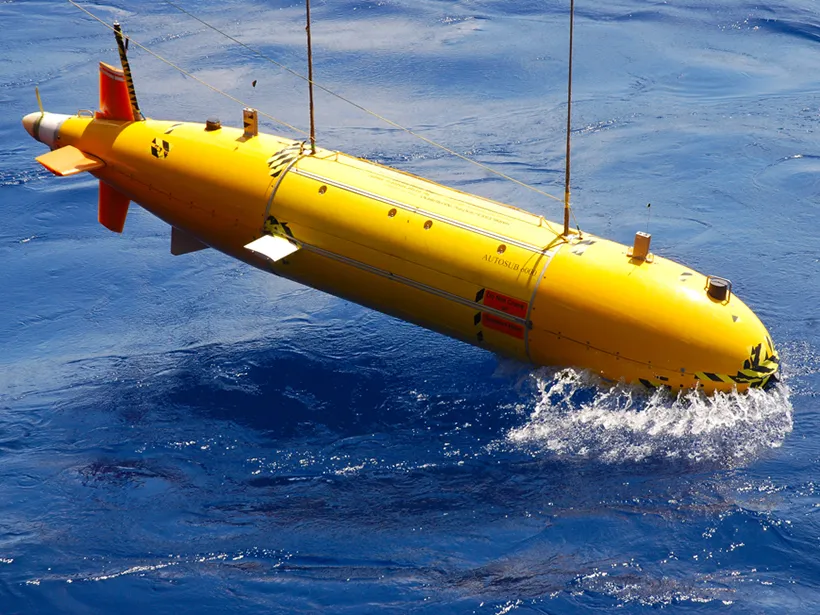
\includegraphics[height = 3.38cm, width=0.8\textwidth]{AUV_2.png}%4.3 metros de comprimento
            \caption{\nocite{REMUS6001:online}}
        \end{figure}
        
        \column{.6\linewidth}
        \begin{figure}
           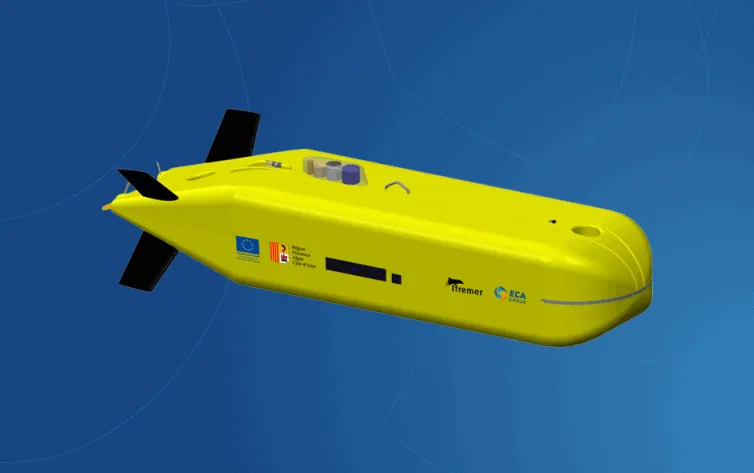
\includegraphics[height = 3.38cm, width=0.6\textwidth]{auv-3.png}%45.7cm de comprimento
            \caption{\nocite{BlueROV210:online}}
        \end{figure}
        
    \end{columns}

%*----------- notes
    \note[item]{Notes can help you to remember important information. Turn on the notes option.}
\end{frame}
%-
%*----------- SLIDE -------------------------------------------------------------
\begin{frame}[t]{Introdução}
    \transboxout[duration=0.5]
    \framesubtitle{História}
    \begin{columns}
        \column{.1\textwidth}
        \column{.4\textwidth}
            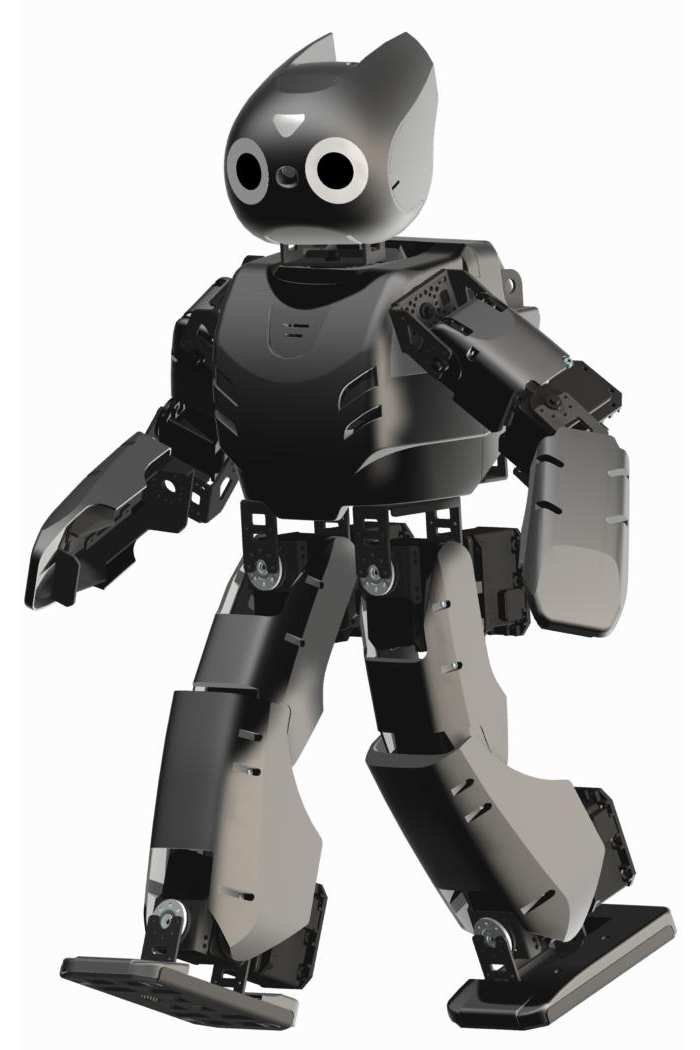
\includegraphics[width=.7\textwidth]{darwin-op}
        \column{.4\textwidth}
            \begin{itemize}
               \item Whintehead torpedo (1866)
               \item Veículo de pesquisa subaquática de propósito especial (1957)
            \end{itemize}
    \end{columns}
 %*----------- notes
    \note[item]{Notes can help you to remember important information. Turn on the notes option.}
\end{frame}
%-